% TODO: 
% Electrodynamics of continuous media
% -> Lorentz-Drude model
% -> Dispersion relation in Lorentz-Drude media
% -> Drude model, conductivity and superconductivity
% Spatial-dispersive model for continuous media
% -> General formulation of spatial dispersion
% -> Magnetic effects included in spatial-dispersive permittivity
% -> Comparison of eps-mu and spatial-dispersive models (electric quadrupoles..., [Merlin])
% -> Why magnetic resonances do not contribute to static permeability?
% Electrodynamics of periodic structures

%% TODO remaining topics to be added: 
%%			* PhCs with metallic/metamaterial inclusios, [Monsoriu, Lina Shi and friends]
%%			* what is MM, what is PhC?
%%			* Kramers-Kronig (in complex plane)

%% TODO sources to be added:

%% TODO time convention

%% """ If a too-simplistic physical theory is forced to predict or explain data that are not within its scope,
%%     it can often do so, but without giving any physical insight. Such a result is not a proof of the theory to be
%%     applicable to the problem, and in some cases not even of the theory to make any sense whatsoever."""

% TODO we refer to tunability - complete it in the rest of the document!!
%% TODO unify impedance as `Z', not `z'

% TODO check if the wavenumber K~/ (2pi/a) is correct
% unify the terminology "band diagram" - "dispersion curves"




% TODO: 
% Electrodynamics of continuous media
% -> Electromagnetic wave in vacuum
% -> Lorentz-Drude model
% -> Dispersion relation in Lorentz-Drude media
% -> Drude model, conductivity and superconductivity
% Spatial-dispersive model for continuous media
% -> General formulation of spatial dispersion
% -> Magnetic effects included in spatial-dispersive permittivity
% -> Comparison of eps-mu and spatial-dispersive models (electric quadrupoles..., [Merlin])
% -> Why magnetic resonances do not contribute to static permeability?
% Electrodynamics of periodic structures
% -> Bloch theorem (and its proof)
% -> K-space and isofrequency contours
% -> Group velocity, phase velocity and their signs [Mikki]
% -> Homogenisation by NRW algorithm, automatic branch selection
% -> Antiresonances -- problems with epsilon-mu approach
% -> EDB model for periodic structures
% Homogenisation algorithms 
% -> PWEM
% -> Reflection-transmission, or NRW, method
% -> Current-driven homogenisation

% Numerical methods used
% -> 


\add{The theoretical chapter starts with a brief review of \textit{electrodynamics of continuous media}. In its customary form without account for spatial dispersion, this topic is treated in every related textbook, so classical linear electrodynamics is introduced in a minimalistic manner, avoiding many relevant topics such as TODO, which are not essential for the description of metamaterials.  This serves as a basis for transforming into the so-called Landau-Lifshitz formulation of electrodynamis for spatially-dispersive media, which is elaborated more in detail.}
\section{Electrodynamics of continuous media} 
\subsection{Electromagnetic wave in vacuum} % FIXME
\paragraph{Maxwell equations} In the realm of classical physics, the electromagnetic phenomena are governed by the \textit{Maxwell equations} in the following form: %{{{
%We assume here that there are no free charges and no currents in the structure: 
\begin{equation} \nabla \cdot  \D = 0, \label{eq_me1}\end{equation}  
\begin{equation} \nabla \cdot  \B = 0, \label{eq_me2}\end{equation}  
\begin{equation} \nabla \times \E = -\frac{\partial \B} {\partial t}, \label{eq_me3}\end{equation}  
\begin{equation} \nabla \times \HH =  \frac{\partial \D} {\partial t}, \label{eq_me4}\end{equation}  
where the $\E$ and $\HH$ are the electric and magnetic vector fields, and $\D$ and $\B$ are the electric and magnetic displacements,
 respectively. These two pairs of field and displacement are related in a similar way as a force is related to the deformation. The \textit{constitutive relations} depend on the properties of the medium the wave propagates in, and in vacuum they take the simplest possible form:
\begin{equation}		\D = \varepsilon_0	\E, \quad\quad\quad						\B = \mu_0			\HH,				 \label{eq_ce}\end{equation}
the $\varepsilon_0 = 8.85\cdot10^{-12}$ F/m being the \textit{vacuum permittivity} and $\mu_0 = 1.25\cdot10^{-6}$ H/m being the \textit{vacuum permeability}. 
Pages \pageref{starttext}--\pageref{endtext} of this thesis will be concerned with computation, interpretation, and experimental verification of the Eq. (\ref{eq_me1}--\ref{eq_me4}) solutions for specific choices of constitutive equations.
\label{starttext}
%}}}
\paragraph{Wave equation in vacuum} The pair of first-order differential equations (\ref{eq_me3}, \ref{eq_me4}) can be converted to a single second-order differential equation. To this end, we apply an extra curl operator $\nabla\times$ from the left, and substituting from one equation into the another, we accumulate two curl operators on the left hand side and two derivatives on the right hand side: %{{{
\begin{equation} \nabla\times (\nabla\times \E) = \nabla\times \left(- \frac{\partial \B} {\partial t}\right) = -\mu_0 \frac{\partial}{\partial t} \left(\nabla\times \HH\right) 
= -\mu_0 \frac{\partial^{2} \D}{\partial t^{2}} = -\mu_0 \varepsilon_0 \frac{\partial^{2} \E}{\partial t^{2}}.  \label{eq_elim}\end{equation}
Using the vector calculus identity
\begin{equation} \nabla\times (\nabla\times \E) \equiv \nabla (\nabla \cdot \E) - \nabla^2 \E, \label{eq_rotrot}\end{equation}
we obtain the \textit{wave equation} for the electric field in vacuum: 
\begin{equation}  \nabla (\nabla \cdot \E) - \nabla^2 \E = -\mu_0 \varepsilon_0 \frac{\partial^{2} \E}{\partial t^{2}}.  \label{eq_wave}\end{equation}
%Note this holds for each component of electric field independently. -- NOT: the divergence is not independent of other components
Starting with Eq. (\ref{eq_me4}) instead of (\ref{eq_me3}), the same result could also be easily obtained for the magnetic field $\HH$.
%}}}
\paragraph{Plane wave and its dispersion relations in vacuum} %{{{
The solutions of the wave equation (\ref{eq_wave}) take the form of a plane harmonic wave in the simplest case, and in any other case the fields can be decomposed as a linear superposition of more such waves and treated separately \cite{jackson1962book}. 

Linear electrodynamics is often treated with the electromagnetic field described as a complex exponential, i.e. as a superposition of two waves differing by a mere quarter-period phase shift, one defining the real part, one the imaginary part of the field. In comparison with the intuitive description of a plane wave in terms of a cosine (or sine) function, the complex notation formally simplifies some mathematical operations, e.g. it allows to easily identify the \textit{phase of a wave as} the exponent (divided by $1/\ii$). In the real world, observable fields do not have any imaginary component so the real part of the result has to be taken. 

An important note shall be made on the sign convention. We use the `engineering' convention $e^{\ii \omega t}$ with wave phase \textit{growing in time}, but this is only due to the author's feeling that it is more intuitive in the literature 
(e.g. \cite[p. 9]{engheta2006book}
\cite[pp. 21, 99]{krowne2007book}
\cite[chap. 1-4, 6, 9, 10]{eleftheriades2005book})
. In roughly a half of the literature
(e.g. \cite{jackson1962book} 
\cite{veselago1968} 
\cite{born1966book}
\cite[chap. 5, 7, 8]{eleftheriades2005book}), the opposite, `optical', convention is used with time dependence of $e^{-\ii \omega t}$. 
The choice of $e^{+\ii\omega t}$ or $e^{-\ii\omega t}$ determines the sign of imaginary part in virtually all complex quantities discussed in this thesis, but with correct interpretation it makes no difference in the physical conclusions.
%% ---- "ENGINEERING" in favor of +iwt , and then perhaps using eps = (eps' - i eps''), or getting along with all-negative eps''
%% https://www.comsol.com/support/knowledgebase/1009/    
%% http://www.tpdsci.com/tpc/RISignDv.php
%% Panofsky & Phillips 1962, p 200 ??
%% ---- "OPTICS" in favor of -iwt, then using the simpler eps = (eps' + i eps'')
%% [noginov2011tutorials, p. 5] has little theory, but uses eps = (eps' + i eps'')
%% ---- 
%% Fourier transform is never subject to the sign change, cf. \ref{eq_kkF}

%% TODO add figure: plane wave
Without loss of generality, we define the electric field as a function of time $t$ and position in space $\rr$, corresponding to a plane wave in the complex notation:
\begin{equation} \E(t, \rr) := \E_0\, e^{\ii\omega t - \ii\kk\cdot\rr} \label{eq_pw}\end{equation}
The plane wave is fully characterised by its \textit{amplitude vector} $\E_0$, \textit{angular frequency} $\omega$ and \textit{wave vector} $\kk$. 
Only some combinations of ($\E_0, \omega, \kk$) provide a physical solution of the wave equation (\ref{eq_wave}). In vacuum, the allowed solutions can be obtained by first substituting the differential operators by their equivalents for a particular plane wave: %TODO explain
\begin{equation} \nabla \rightarrow -\ii\kk, \quad\quad\quad 
\frac{\partial} {\partial t} \rightarrow \ii\omega, \label{eq_difftok}\end{equation}
so the wave equation (\ref{eq_wave}) can be modified the following way:
$$					\nabla (\nabla \cdot \E) - \nabla^2 \E				  =	-\mu_0 \varepsilon_0 \frac{\partial^{2} \E}{\partial t^{2}},  $$
$$				 -\ii\kk (-\ii\kk \cdot \E)  - (-\ii\kk \cdot -\ii\kk) \E = -\mu_0 \varepsilon_0 (\ii\omega)^2 \E, $$
\begin{equation}   - \kk (\kk \cdot \E)      +          k^2 \E            = +\mu_0 \varepsilon_0 \omega^{2} \E.  \label{eq_wavek}\end{equation}
Generally, the branches  of solutions of this equation divide into two groups: % todo proof?
\begin{enumerate}
 \item{\textit{Transverse electromagnetic waves}, with the electric field and wave vector being perpendicular, i.e. $(\kk \cdot \E) = 0$. Therefore, the \textit{dispersion relation} for a transverse plane wave in vacuum is linear:
\begin{equation} k~= \sqrt{\mu_0 \varepsilon_0}\; \omega = \frac{\omega}{c}, \label{eq_dispeq_vac}\end{equation}
where we defined the \textit{speed of light} $c := \frac{1}{\sqrt{\mu_0 \varepsilon_0}}$.
} 
 \item{\textit{Longitudinal electromagnetic waves}, with $\kk\,|| \pm \E$, require the right side of Eq. \ref{eq_wavek} to be zero. A homogeneous static electric field ($k = 0, \omega = 0$) can be considered to be their only solution in vacuum. The following chapters will give some examples of media which support propagating longitudinal waves.} 
 \end{enumerate}
%% TODO add figure: dispersion relation
%}}}

\subsection{Local response of media to the electromagnetic field} \label{loc_response_of_media}
\paragraph{Local response}  %{{{
\label{subsection_local_resp}
In the whole chapter, we expect the medium properties to be time-invariant, linear, and homogeneous (i.e. independent of time, field amplitude and position in space, respectively). 
In this section, we focus on the special case when the medium response in point $\rr$ is not influenced by the electric field in any other point $\brho \neq \rr$. The medium is then said to be \textit{local}. 
For most natural homogeneous media, this approximation is very close to reality and thus numerous electrodynamics textbooks tend to omit the nonlocal effects. 
However using this local theory to a wave propagating through periodic structures has a priori no justification and may lead to completely wrong results. The local theory presented here will serve as a basis for the nonlocal theory developed in following chapters.
% Applying the more familiar local electrodynamics to these structures is a mistake common to many papers. While the local theory is mathematically consistent, it predicts unusual spectral shapes and does not allow their further physical interpretation.

When an electric field $\E$ is applied, the medium responds by a change of the electric displacement $\D$ in a way that is characteristic for it. 
The immediate response of vacuum from the right side of the constitutive equations (\ref{eq_ce}) remains unchanged, but the response of the matter adds a new term called \textit{electric polarisation}. The polarisation is not instantaneous, so it is generally expressed as a convolution of the \textit{electric susceptibility} $\chi_e^{\rm(Loc)}$ with the values of electric field in the previous time $\tau$:
\begin{equation} \D(t,\rr) = \varepsilon_0 \E(t,\rr) + \varepsilon_0 \int_{-\infty}^{t}\chi_e^{\rm(Loc)}(t-\tau)\, \E(\tau,\rr)\,\mbox{d}\tau. \label{eq_loc_chi_convol}\end{equation}
\add{
Assume that a harmonic plane wave propagates through the medium, so $\E(t, \rr) := \E_0 \, e^{\ii\omega t - \ii\kk\cdot\rr}$, as given by Eq. (\ref{eq_pw}). This can be inserted in the above equation:
\begin{equation} \D(t,\rr) = \varepsilon_0 \E_0 \, e^{\ii\omega t - \ii\kk\cdot\rr} + \varepsilon_0 \int_{-\infty}^{t} \chi_e^{\rm(Loc)}(t-\tau) \, \E_0 \, e^{\ii\omega \tau - \ii\kk\cdot\rr} \,\mbox{d}\tau. \label{eq_chi_convol_harm}\end{equation}
Substituting $T:=t-\tau$, the exponent can be separated into two parts: one of which factors out of the integrals, and the remaining part that turns the convolution into a temporal Fourier transform of the medium response:
$$				 \D(t,\rr) = \varepsilon_0 \E_0 \, e^{\ii\omega t - \ii\kk\cdot\rr} + \varepsilon_0 \int_{-\infty}^{0} \chi_e^{\rm(Loc)}(T) \, \E_0 \, e^{\ii\omega (t - T) - \ii\kk\cdot\rr} \,\mbox{d}T,$$
$$				 \D(t,\rr) = \varepsilon_0 \E_0 \, e^{\ii\omega t - \ii\kk\cdot\rr} + \varepsilon_0 \left( \int_{-\infty}^{0} \chi_e^{\rm(Loc)}(T)  \, e^{-\ii\omega T}\,\mbox{d}T  \right) \E_0 \, e^{\ii\omega t - \ii\kk\cdot\rr}.$$
This is nothing but an application of the convolution theorem: convolution in time domain is equivalent to multiplication in frequency domain.  %% FIXME normalisation by 2pi?
Consequently we may introduce the local \textit{relative permittivity} $\varepsilon_r^{\rm(Loc)}(\omega)$ as a function of frequency. It is a property of the medium that determines how strong it develops the electric displacement $\D$ in response to a harmonic wave. From Eq. (\ref{eq_ce}) it is clear that in vacuum,  $\varepsilon_r^{\rm(Loc)} = 1$.
\begin{equation}  \varepsilon_r^{\rm(Loc)}(\omega) =   \frac{\D(t,\rr)}{\varepsilon_0 \E(t,\rr)} \biggr|_{\E(t, \rr) := \E_0 \, e^{\ii\omega t - \ii\kk\cdot\rr}} = 1 + \int_{-\infty}^{0} e^{-\ii\omega T} \,\chi_e^{\rm(Loc)}(T) \,\mbox{d}T \label{eq_eps_loc}\end{equation}
%% TODO note that this is a complex-valued function, unlike chi_e(loc); and explain why it is so: that it allows to easily pack in also the information about the phase
The response function $\chi_e(T, \mathbf{R})$ of usual media is composed of different phenomena.
Each of them may react on different time scales, and thus the medium response usually has a relatively complicated shape in the time domain. 
However, to a reasonable degree of approximation, each of the contributions can be modelled as a harmonic oscillator, as is demonstrated in the following.
% The corresponding function $\varepsilon^{\rm(Loc)}(\omega)$ in the frequency domain allows to identify the effects in a clearer way.
% : the electrons around an atomic nucleus can slightly displace from their initial position around the nucleus, and so can the charged atoms from their equilibrium position the lattice; polar molecules (if present) can reorient their dipoles and other more subtle contributions may occur.
}
%}}}
\paragraph{Response of a harmonic oscillator} \label{chap_lorentzmedia} %{{{
\begin{figure}[t] \caption{\textbf{a)} Illustration of how a simplified medium may respond to an electric field impulse in the shape of Dirac delta function  $E(t) = \delta(t)$. The response of  is composed from an instantaneous part from vacuum, $\delta(t)$, and from a delayed ringdown of one damped harmonic oscillator, described by $\chi_e^{\rm(Loc)}(t) := 2\pi \sin(2\pi t)\,e^{-x/2}$; \textbf{b)} The corresponding local permittivity $\epsrl(\omega)$, computed by Fourier transform of the response. Note that the imaginary part of permittivity is negative due to that the material is lossy (absorbs energy) and that the $e^{\ii\omega t}$ convention is used.} \label{fg_oscillator_spectrum} \centering 
	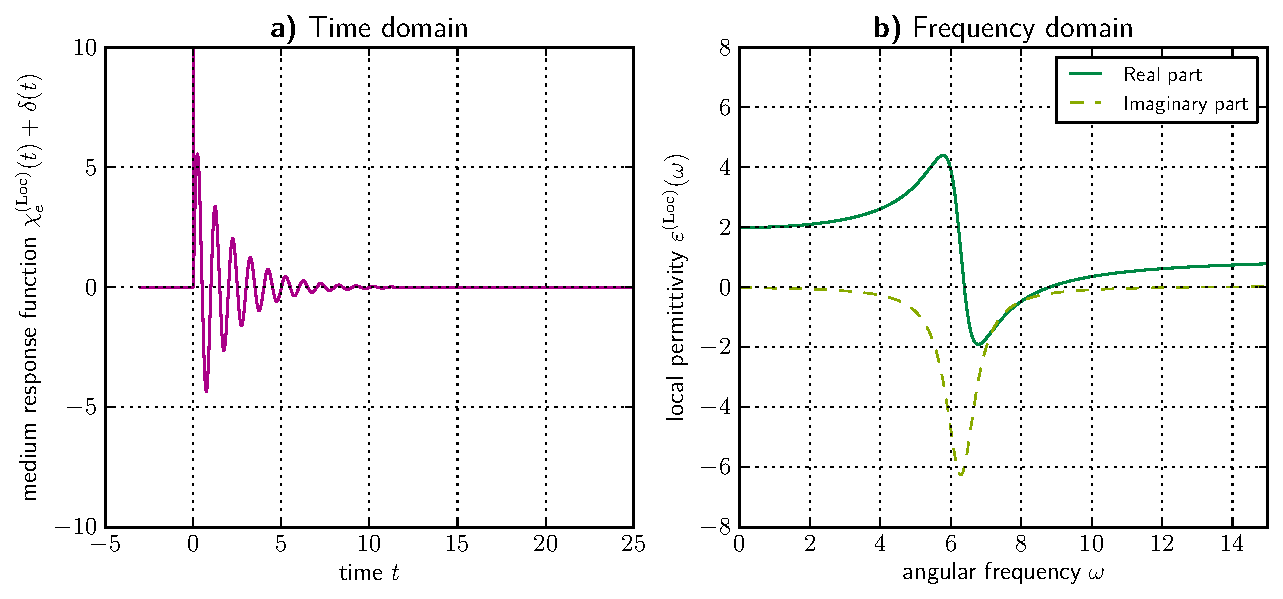
\includegraphics[width=15cm]{img/oscillator_spectrum.pdf}
\end{figure}
Linear physical systems with an inertial mass, friction force and a restoring force are known as \textit{damped harmonic oscillators}. 
This theory applies well to the electrons elastically bound to an atomic nucleus, as well as to the atoms elastically bound to their equilibrium position in the lattice. The molecular rotation can also be modelled as an (possibly overdamped) harmonic oscillator. Even the free electrons in conductive media can fit into the theory of harmonic oscillator provided the restoring force is set to nearly zero. The response of a harmonic oscillator is easy to describe both in time domain and frequency domain, even without the explicit use of the Fourier transform from Eq. (\ref{eq_eps_loc}). The harmonic oscillator model thus becomes a convenient starting point to approximate the response of materials.

Any damped harmonic oscillator is described by a second-order differential equation:
\begin{equation} \alpha \frac{\partial^{2} x(t)}{\partial t^{2}} + \beta\frac{\partial x(t)}{\partial t} + \zeta x(t) = f(t). \label{eq_harm_osc}\end{equation}
Provided the driving term on the right hand side  is harmonic $f(t) = e^{+\ii \omega t}$, the system response is also a harmonic function, $x(t) = \chi(\omega) e^{+\ii \omega t}$. The differential equation (\ref{eq_harm_osc}) can be easily solved to show that the complex amplitude of the driven oscillations, $\chi(\omega)$, depends on the angular frequency and on the parameters $\alpha$, $\beta$ and $\zeta$ in the following way:
\begin{equation} \chi(\omega) \equiv \frac{x(t)}{f(t)} = \frac{1}{\zeta-\alpha\omega^{2} + \ii\omega\beta}  = \frac{\alpha^{-1}}{\frac{\zeta}{\alpha}-\omega^{2} + \ii\omega\frac{\beta}{\alpha}}. \label{eq_harm_osc_result}\end{equation}
The physical meaning of $\alpha$, $\beta$ and $\zeta$ is of little importance in this text, but without loss of generality the result of Eq. (\ref{eq_harm_osc_result}) can be rewritten into
\begin{equation} \chi(\omega) = \frac{F}{\omega_0^{2}-\omega^{2} + \ii\omega\gamma}, \label{eq_harm_osc_rewritten}\end{equation}
where the physical interpretation of the three (real and positive) parameters is as follows:
\begin{itemize}
 \item{$\omega_0 = \sqrt{\zeta/\alpha}$ is the angular \textit{frequency of resonance}, at which the response is pure imaginary and usually its modulus $|\chi(\omega=\omega_0)|$ is near its maximum.} 
 \item{$\gamma = \zeta/\alpha$ is the \textit{damping rate}. In time domain, it determines the time constant of exponential amplitude decay. In frequency domain, it is roughly proportional to the resonance width. } 
 \item{$F = \alpha^{-1}$ is the \textit{oscillator strength}, determining the amplitude of the response function.}
 \end{itemize}

\paragraph{Permittivity of Lorentz media} Within the approximation of relatively weak fields, the oscillators act independently of each other.
The response of usual media in frequency domain can thus be decomposed with acceptable precision into a sum of $M$ independent harmonic oscillators, each $m$-th oscillator having the resonance angular frequency $\omega_{0m}$, damping rate $\gamma_m$ and strength $F_m$.
The permittivity function of the material is a solution of the differential equation of a damped harmonic oscillator, driven by a harmonic source:
\begin{equation} \epsrl(\omega) = 1 + \sum_{m=1}^M \frac{F_m}{\omega_{0m}^2 - \omega^2 + \ii\omega\gamma_m} \label{eq_lorentz_eps}\end{equation} %% TODO fix sign; TODO what about eps0 before summation?
Advancing from the general formulation in Eq. (\ref{eq_eps_loc}) to the Lorentz oscillator model in Eq. (\ref{eq_lorentz_eps}) if of great importance for theoretical interpretation of the material response, and it has also become a framework for description of periodic structures even in the presence of spatial dispersion. 
% It is also the way how one communicates the material definition to the numerical simulation software, as described later (in Chap. \ref{chap_fdtd}). 
% TODO decide whether we use exp(i omega t)     -> leads to negative eps''

One can see that each oscillator increases the real part of permittivity, but in the high frequency limit the contribution of the oscillator vanishes. This can be intuitively understood as that at low frequencies $\omega \ll \omega_0$, the system reacts fast enough to simultaneously follow the driving force, whereas at high frequencies  $\omega \gg \omega_0$, the system does not follow the driving force at all.
The contribution of one oscillator to the low-frequency permittivity $\Delta\varepsilon_r(0)$, is inversely proportional to the oscillator restoring force, which links it to the inverse square of the resonance frequency:
\begin{equation} \Delta \varepsilon_r'(\omega\rightarrow0) = \frac{F}{\omega_0^{2}}.  \label{eq_delta_eps} \end{equation}

A more detailed treatment of the theory of the dielectric function $\epsrl(\omega)$ may be found in many textbooks, e.g. \cite[p. 454]{klingshirn2007semiconductor}, \cite{dresselhaus1966optical}. 

We will return to the Lorentz oscillator model also in the Chapter \ref{def_of_mat}, where the shows to be essential for realistic definition of materials for accurate numerical FDTD simulations. The chapter also describes in more detail how the overdamped molecular rotation and the unbound motion of free charges can be easily represented using correct parameters of an oscillator.
%}}}
\paragraph{Permeability of Lorentz media}  %{{{ 
In a manner very similar to the above derivation of the local permittivity, the \textit{local permeability} can be introduced by means a response of the medium to the magnetic field:
\begin{equation} \mu^{\rm(Loc)}(\omega) = \frac{\B(t,\rr)}{\mu_0\HH(t,\rr)} \biggr|_{\HH(t, \rr) := \HH_0 \, e^{\ii\omega t - \ii\kk\cdot\rr}} = 1 + \int_{-\infty}^{0} e^{-\ii\omega T} \,\chi_m^{\rm(Loc)}(T) \,\mbox{d}T, \label{eq_mu_loc}\end{equation}
where $\chi_m^{\rm(Loc)}(T)$ is the \textit{magnetic susceptibility of medium} and $\HH_0$ is the amplitude of the magnetic field. This obviously results in an expression for the local permeability in the frequency domain:
\begin{equation} \murl(\omega) = 1 + \sum_{m=1}^M \frac{F_m}{\omega_{0m}^2 - \omega^2 + i\omega\gamma_m}, \label{eq_lorentz_mu}\end{equation} %% TODO fix sign; TODO what about eps0 before summation?
where formally the same notation was used as in  Eq. (\ref{eq_lorentz_eps}): $\omega_{0m}$, $\gamma_m$ and $F_m$ are the magnetic oscillator's angular frequency, damping frequency and strength. Unlike the electric response, most ordinary media have either almost no response to the magnetic field % todo CITE
or their response is limited to low frequencies.

%}}}
\paragraph{Kramers-Kronig relations in local media}%{{{
Causality prevents any medium from reacting to the future electric (or magnetic) field, so the integration in Eq. (\ref{eq_loc_chi_convol}) goes up to the current time only, $\tau \in (-\infty, t)$. The response of the medium to a real-valued field must moreover be also real, no matter that the computations are often done with complex field amplitude [Eq. (\ref{eq_pw})] for the sake of convenience. 

Thus, the basic physical laws impose relatively strict constraints to the time-domain response function $f(t)$, which translate into another constraints for the possible shape of the response in frequency domain $F(\omega)$. The intuitive physical derivation is based on the fact that any time-domain response function can be trivially separated into its odd and even parts as 
, as shown in Fig. \ref{fg_kk}. 
\begin{equation}f(t) = f_{odd}(t) + f_{even}(t) = -f_{odd}(-t) + f_{even}(-t) \label{eq_odd_even_decomp}\end{equation}
\begin{figure}[t] \caption{Illustration of how a real causal function $f(t)$ can be decomposed into the odd and even parts, which then yield a pure imaginary and pure real functions in the spectrum, respectively. Mathematically this is expressed in Eqs. (\ref{eq_odd_even_decomp}--\ref{eq_kkresult}).} \label{fg_kk} \centering 
	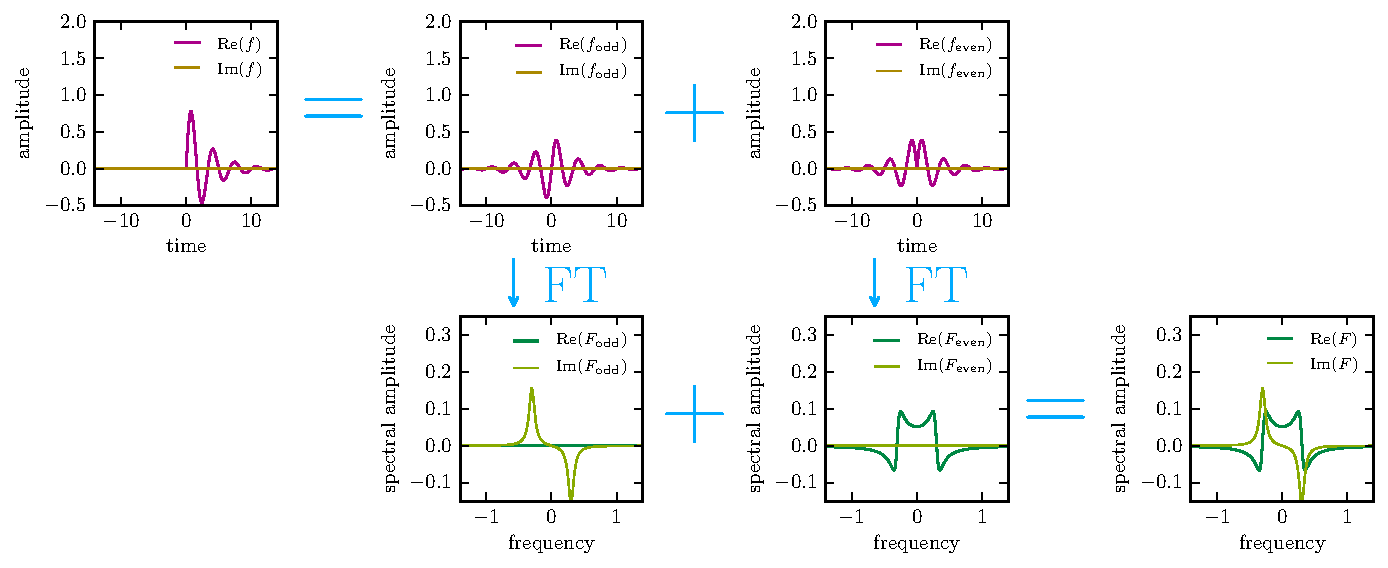
\includegraphics[width=17.5cm]{img/Kramers_Kronig_plot/kk.pdf}
\end{figure}
The Fourier transform of a real odd function is an imaginary function:
%F_{odd}(\omega)=& \int_{-\infty}^{\infty} e^{-\ii \omega t} f(t) \mbox{d}t = \\
		 %=&  \frac{1}{2} \int_{0}^{\infty} e^{-\ii \omega   t } [ f_{odd}(t) + f_{even}(t)] \mbox{d}t 
		   %+ \frac{1}{2} \int_{0}^{\infty} e^{-\ii \omega (-t)} [-f_{odd}(t) + f_{even}(t)] \mbox{d}t  \\
		 %=&  \int_{0}^{\infty} \frac{e^{-\ii \omega t}-e^{+\ii \omega t}}{2} f_{odd}(t) \mbox{d}t 
		   %+ \int_{0}^{\infty} \frac{e^{-\ii \omega t}-e^{+\ii \omega t}}{2} f_{odd}(t) \mbox{d}t  = \\
		 %=&\int_{-\infty}^{\infty} e^{-\ii \omega t} f(t) \mbox{d}t  = \\
		 %=&\int_{-\infty}^{\infty} e^{-\ii \omega t} f(t) \mbox{d}t  = \\
\begin{equation} 
\begin{split} 
F_{odd}(\omega)=& \int_{-\infty}^{+\infty} e^{-\ii \omega t} f_{odd}(t) \,\mbox{d}t = 
		 \int_{-\infty}^{+\infty} \frac{e^{-\ii \omega   t }}{2} f_{odd}(t) \,\mbox{d}t 
		   +  \int_{-\infty}^{+\infty} \frac{e^{-\ii \omega (-t)}}{2} [-f_{odd}(-t)] \,\mbox{d}t  \\
		 =&   \int_{-\infty}^{+\infty} \frac{e^{-\ii \omega t}-e^{+\ii \omega t}}{2} f_{odd}(t) \,\mbox{d}t 
		 = -\ii \underbrace{\int_{-\infty}^{+\infty} \sin(\omega t) \, f_{odd}(t) \,\mbox{d}t}_{\mbox{$\in \mathbb{R}$}},
\end{split} 
\label{eq_kkF}\end{equation}
whereas the Fourier transform of a real even function yields a real function:
\begin{equation} 
\begin{split} 
F_{even}(\omega)= \ldots =   \int_{-\infty}^{+\infty} \frac{e^{-\ii \omega t}+e^{+\ii \omega t}}{2} f_{even}(t) \,\mbox{d}t 
		 = \underbrace{\int_{-\infty}^{+\infty} \cos(\omega t) \, f_{even}(t) \,\mbox{d}t}_{\mbox{$\in \mathbb{R}$}}.
\end{split} 
%% TODO the following is WRONG! see ---->  http://www.thefouriertransform.com/pairs/step.php#signum,  ho3.pdf
\label{eq_kkFeven}\end{equation}
The odd and even components of the time-domain response function correspond to the imaginary and real part of the response spectrum, respectively:
\begin{equation} F_{odd}(\omega) + F_{even}(\omega) = F(\omega), \text{ where } F_{odd}(\omega) = F''(\omega) \text{ and } F_{even}(\omega) = F'(\omega).  \label{eq_kkFodd}\end{equation}
At the same time, $f_{even}(t)$ and $f_{odd}(t)$ are related by having the opposite sign for $t<0$ and the same sign for $t>0$, that is 
\begin{equation} f_{even}(t) = \mbox{sign}(t)\,f_{odd}(t). \label{eq_kkfeven}\end{equation}
Multiplication in the time domain manifests as a convolution in frequency domain
\begin{equation} 
F_{even}(\omega) = \int_{-\infty}^{+\infty}  \frac{-2\ii}{\omega - \Omega} F_{odd}(\omega) \,\mbox{d}\Omega  \equiv  \left[\frac{-2\ii}{\omega}\right]\,\ast\,F_{odd}(\omega),
\label{eq_kkresult}\end{equation} 
where we used the knowledge that the $-2\ii/\omega$ function is the Fourier transform of $\mbox{sign}(t)$. Convolution with this function is also known as the Hilbert transform.% tODO cite

Obviously, Eq. (\ref{eq_kkfeven}) can also be converted to $f_{odd}(t) = \mbox{sign}(t)\,f_{even}(t)$, thus the relation between the real and imaginary part of the response spectrum also holds when $F_{odd}(\omega)$ and $F_{odd}(\omega)$ are exchanged in Eq. (\ref{eq_kkresult}). 

A related mathematical proof of Kramers-Kronig relations can be derived from the analytic properties of the response function in the complex plane.

%% TODO: why do K-K relations forbid to choose arbitrary phase difference over an unit cell? 
%% ie. Why the Neff can be unambiguously extracted from spectra?
% TODO show how it dictates the "constant area of imaginary part " when resonance Q is changed
%}}}
\subsection{Dispersion relations in local Drude-Lorentz media} \label{disp_rel_local_media}
% TODO Two questions: why omega_p had to be normalized by sqrt 2pi and why limit of hi-freq sigma'' had to be divided by 2pi?
\paragraph{Lower and upper polariton branches}  % TODO%{{{
%}}}
\paragraph{Resonance in magnetic permeability}  % TODO%{{{
%}}}
\paragraph{Negative phase velocity of doubly-negative media}  % TODO%{{{
%}}}

\subsection{Nonlocal response} % TODO
%{{{
The previous two chapters that concerned local media were included mostly for a comparison with the nonlocal theory that follows.
In this section a more general class of media is discussed, where the polarization explicitly depends the history of $\E(\tau, \brho)$ in previous time $\tau < t$ and in all surrounding points $\brho$, and therefore is described by a spatio-temporal convolution:
\begin{equation} \D(t,\rr) = \varepsilon_0 \E(t,\rr) + \varepsilon_0\int_{V} \int_{-\infty}^{t} \chi_e(t-\tau, \rr-\brho) \, \E(\tau,\brho) \,\mbox{d}\tau \,\mbox{d}^3\brho. \label{eq_chi_convol_nonloc}\end{equation}
\mdf{
In a very similar manner as in the local theory above, we expect a plane wave $\E(t, \rr) := \E_0 \, e^{\ii\omega t - \ii\kk\cdot\rr}$ propagates through the medium. 
\begin{equation} \D(t,\rr) = \varepsilon_0 \E_0 \, e^{\ii\omega t - \ii\kk\cdot\rr} + \varepsilon_0\int_{V} \int_{-\infty}^{t} \chi_e(t-\tau, \rr-\brho) \, \E_0 \, e^{\ii\omega \tau - \ii\kk\cdot\brho} \,\mbox{d}\tau \,\mbox{d}^3\brho. \label{eq_chi_convol_harm_nonloc}\end{equation}
After two  substitutions, $T:=t-\tau$, $\mathbf{R}:=\rr-\brho$, the exponent can again be separated into the original plane wave (that factors out), and a spatio-temporal Fourier transform of the medium response:
$$				 \D(t,\rr) = \varepsilon_0 \E_0 \, e^{\ii\omega t - \ii\kk\cdot\rr} + \varepsilon_0\int_{V} \int_{-\infty}^{0} \chi_e(T, \mathbf{R}) \, \E_0 \, e^{\ii\omega (t - T) - \ii\kk\cdot(\rr - \mathbf{R})} \,\mbox{d}T \,\mbox{d}^3\brho,$$
$$				 \D(t,\rr) = \varepsilon_0 \E_0 \, e^{\ii\omega t - \ii\kk\cdot\rr} + \varepsilon_0\left( \int_{V} \int_{-\infty}^{0} \chi_e(T, \mathbf{R})  \, e^{-\ii\omega T + \ii\kk\cdot \mathbf{R}}\,\mbox{d}T \,\mbox{d}^3 \mathbf{R} \right) \E_0 \, e^{\ii\omega t - \ii\kk\cdot\rr}.$$
The response of the medium to the electric field of any harmonic plane wave can now be expressed as a function of frequency $\omega$ and wave vector $\kk$. It is defined as the ratio between the electric displacement and the electric field:
\begin{equation} \varepsilon_r(\omega, \kk) = \frac{\Dsd(t,\rr)}{\varepsilon_0 \E(t,\rr)} \biggr|_{\E(t, \rr) := \E_0 \, e^{\ii\omega t - \ii\kk\cdot\rr}} = 1 + \int_{V} \int_{-\infty}^{0} \chi_e(T, \mathbf{R}) \,e^{-\ii\omega T + \ii\kk\cdot \mathbf{R}} \,\mbox{d}T \,\mbox{d}^3\mathbf{R} \label{eq_eps_nonloc}\end{equation}
%% TODO think over - we substituted Dsd for D    and    eps for eps^(Loc) , but the new epsilon is not that one containing magnetic effects as in Landau-Lifshitl.
%%	 We must tell apart eps and eps^LL
%%						... should not the notation be unified for clarity? 
%%						... and when it happens that eps == eps^(Loc) ?? And when eps^LL== eps^(Loc)
Converting the problem from spatio-temporal domain into the wavenumber-frequency domain allows to express the relation between $\D$ and $\E$ by the \textit{permittivity} function $\varepsilon(\omega, \kk)$ and completely avoid the convolution from Eq. (\ref{eq_chi_convol_nonloc}). Note that both the response function $\chi_e$ and the permittivity $\varepsilon$ may be either scalar functions, or rank-2 tensor functions; the latter case accounts for possible anisotropy of the medium.
% , and convolution in space is equivalent to multiplication  in the reciprocal space
}



\subsection{Comparison to local response} \add{TODO}
Note the response function for a local medium can be formally derived from its nonlocal formulation by replacing the spatial dependence by a Dirac delta function: %% TODO fix the sencence - it is in fact incorrect
\begin{equation} \chi_e(t-\tau, \rr-\brho) = \delta^{3}(\rr-\brho) \; \chi_e^{\rm(Loc)}(t-\tau), \label{eq_loc_chi}\end{equation}
which allows to simplify Eq. (\ref{eq_chi_convol}) in the way that in local media only the temporal convolution has to be computed.

% TODO The exact shape of $\varepsilon(\omega, \kk)$ will be discussed later.
%}}}
\subsection{Dispersion relations in nonlocal media} % TODO
\paragraph{Review of local medium parameters}%{{{
Some phenomena observed in the frequency spectrum are in fact consequences of spatial dispersion, such as Doppler broadening of resonance lines in gases.\cite[p. 359]{landau1984electrodynamics} More precisely, these phenomena are primarily dependent on the wave vector $\kk$, and their expression by means of the temporal spectrum is a mere approximation based on that the dispersion curve usually defines a simple relation between  frequency and wave vector. 

The above chapter \ref{disp_rel_local_media} presented the customary approximation of local media, where the electric permittivity in Eq. (\ref{eq_eps_loc}) is composed of two terms: 
\begin{enumerate}
 \item{one caused  by the immediate response of vacuum,} 
 \item{and another by the electric response of matter.}
 \end{enumerate}
In a very similar way, the local magnetic permeability $\murl(\omega)$ also consists of two different components, 
\begin{enumerate}[resume]
 \item{the magnetic response of vacuum,} 
 \item{and, if present, the magnetic response of the matter.} 
\end{enumerate}
\begin{table}[ht]   \caption{}  \label{tb_} \centering 
\begin{tabular}{lcr}
 \toprule
Physical effect & Has corresponding term in \\
 \hline
Vacuum permittivity &	&	\\
 &	&	\\
Vacuum permeability &	&	\\
 &	&	\\
 \bottomrule
 \end{tabular} \end{table}


The trivial extension of the local medium description to the nonlocal one could consist in redefining both constitutive parameters as functions of frequency and wave vector: $\varepsilon_r(\omega) \stackrel{?}{\rightarrow} \varepsilon_r(\omega, \kk)$, $\mu_r(\omega) \stackrel{?}{\rightarrow} \mu_r(\omega, \kk)$, but this will not be used. 
%}}}

\paragraph{Magnetic effects can be described by electric displacement}%{{{
Instead, we will show here that the magnetic response can be fully expressed by a certain form of $\varepsilon_r(\omega, \kk)$ dependence on $\kk$. In the following theory, the spatial-dispersive function $\varepsilon_r(\omega, \kk)$ will consist of
\begin{enumerate}
 \item{the component caused by the immediate electric response of vacuum,} 
 \item{the component caused by the electric response of matter,}
 \item{and a new component fully accounting for the \textit{magnetic} response of matter, thanks to a particular shape of its spatial dispersion.}
\end{enumerate}
The magnetic permeability $\mu_r$ becomes a mere constant of
\begin{enumerate}[resume]
 \item{the magnetic response of vacuum [as in Eq. (\ref{eq_ce})].} 
\end{enumerate}
Additionally, the spatial dispersion allows to describe
\begin{enumerate}[resume]
 \item{other phenomena that can not be described by the local theory.} 
\end{enumerate}
Repeating the Maxwell equation (\ref{eq_me4}) that links the magnetic field $\HH$ with the electric induction $\D$, 
$$ \nabla \times \HH =  \frac{\partial \D} {\partial t},\quad\quad\quad\quad\quad\text{(\ref{eq_me4} again)}$$
it is clear that if one defines new pair of vector fields
\begin{equation} \HHsd = \HH + \frac{\partial\mathbf{X}}{\partial t}, \label{eq_HHsd}\end{equation}
\begin{equation} \Dsd  = \D  + \nabla\times \mathbf{X}, \label{eq_Dsd}\end{equation}
then Eq. (\ref{eq_me4}) maintains exactly the same form with the new fields, for any differentiable vector field $\mathbf{X}$:
\begin{equation} \nabla \times \HHsd = \nabla \times \HH + \left(\nabla\times \frac{\partial\mathbf{X}}{\partial t}\right) = \frac{\partial \D}{\partial t}+ \frac{\partial(\nabla\times \mathbf{X})}{\partial t} =  \frac{\partial \Dsd} {\partial t}, \label{eq_me4sd} \end{equation}
because for well behaved functions the temporal and spatial derivatives commute.

With the freedom of choice of $\mathbf{X}$, we impose the above mentioned requirement that whole magnetic response of the matter is expressed by the constitutive equation for permittivity. Therefore in spatial-dispersive theory, the constitutive equation %% TODO reference some text from above pargraphs
for magnetic induction is defined the same as in vacuum:
\begin{equation} \mu_0 \HHsd := \mu_0 \murl \HH = \B. \label{eq_mu_sd}\end{equation}
When this equation is rearranged into the form similar to \ref{eq_HHsd}, we obtain a prescription for sought $\mathbf{X}$: 
$$ \HHsd = \HH + (\murl -1)\HH = \HH + \underbrace{\left(\frac{\murl-1}{\mu_0\murl}\right)\B}_{=:\,\partial\mathbf{X}/\partial t}$$
Without loss of generality, we again restrict the discussion to a plane wave (\ref{eq_pw}), thus the time derivative equals to multiplication by $\ii\omega$.
\begin{equation} \mathbf{X} = \frac{1}{\ii\omega}\left(\frac{\murl-1}{\mu_0\murl}\right)\B = \frac{1}{\ii\omega\mu_0}\left(1 - \frac{1}{\murl}\right)\B. \label{eq_Xsd}\end{equation}
The new electric displacement $\Dsd$ that also accounts for magnetic phenomena is obtained by substitution of Eq. (\ref{eq_Xsd}) into Eq. (\ref{eq_Dsd}):
\begin{equation} \Dsd := \D - \ii\kk\times \mathbf{X} =  \D - \ii  \frac{1}{\ii\omega\mu_0}\left(1 - \frac{1}{\murl}\right) \kk\times \B  \label{eq_Dsd2}\end{equation}
By means of the other Maxwell equation (\ref{eq_me3}), the magnetic induction $\B$ can be substituted by $\kk\times\E / \omega$ to obtain an expression that contains only the electric quantities.
\begin{equation} \Dsd = \D - \frac{1}{\omega^2 \mu_0}\left(1 - \frac{1}{\murl}\right) \kk\times(\kk\times \E)  \label{eq_Dsd3}\end{equation}
%}}}
\paragraph{Tensor form of the spatial-dispersive permittivity}%{{{
Continuing in the derivation outlined in \cite{landau1984electrodynamics, krowne2007book_agran, agranovich2006spatial}, we can derive the tensor form of spatial-dispersive permittivity $\varepsilon_{ij}(\omega,\kk)$.

The downsides of the spatial-dispersive model of media is that it is more complicated, leading e.g. to implicit dispersion equation. Its great advantage is however that it provides a correct description of periodic structures discussed below. 
%}}}
\paragraph{Comparison of eps-mu and spatial-dispersive models}%{{{
... en vacuum ...
\begin{equation}		\Dsd = \varepsilon_0	\E, \quad\quad\quad						\B = \mu_0			\HHsd,				 \label{eq_ce_dispersive}\end{equation}
%}}}
\paragraph{How a local dielectric manifests in the spatial-dispersive model}  % TODO%{{{
 %(electric quadrupoles..., [Merlin])
%}}}
\paragraph{Why magnetic resonances do not contribute to static permeability?}%{{{
\add{and why high-frequency diamagnetism does not break causality? cite [skaar2014]}
%}}}

\section{Electromagnetic waves in periodic structures}
\subsection{(The mathematical problem)}
%In a given time the wave in a periodic medium takes on the form of Bloch wave (\ref{eq_bloch}): 
 %$\mathbf{E}(\mathbf{r}) = \mathrm{e}^{\mathrm{i}Kz} \cdot \mathbf{u}(\mathbf{r})$, i.e. it is a product of a harmonic \textit{envelope} and a cell-periodic \textit{mode}. Computing the dispersion curves involves computing the envelope wavenumber $K = K(f)$ for each frequency $f$ in the desired spectrum. The information about the mode $\mathbf{u}(\mathbf{r})$ is not used and instead the metamaterial cell is treated as if it was a homogeneous medium -- therefore this procedure is also called \textit{homogenisation}.

\paragraph{The Bloch-Floquet theorem}%{{{
% TODO define periodicity

The important Bloch-Floquet theorem states that while the wave in periodic medium does not have to be periodic anymore, it is a product of two periodic functions:
\begin{equation} \E(t, \rr) = \mathrm{e}^{\mathrm{i} Kz - 2\pi \mathrm{i} f t} \cdot \mathbf{u}(\rr), \text{ where } \mathbf{u}(\rr) = \mathbf{u}(\rr+a\mathbf{z}) = \mathbf{u}(\rr+2a\mathbf{z}) = \ldots, \label{eq_bloch}\end{equation} 
The $\mathbf{u}(\rr)$ function has the same periodicity as the structure. It is generally a complex vector function so it not only alters the direction and magnitude of $\E$ (or  $\HH$), but can also introduce a \textit{phase modulation} of the wave in each unit cell. Note that the capital $K$ is used to distinguish the wavenumber of the Bloch wave envelope from the wavenumber $k$ in free space. Note this theorem does not determine how the shape of $\mathbf{u}(\rr)$ nor the direction and magnitude of $\KK$, it only states they do exist.
% TODO proof /home/filip/PhD/Sources_MM_theory/Bloch_Theorem_Proof.pdf
% TODO example illustration of Bloch wave -> plotted in Python
%}}}
% -> Bloch theorem (and its proof)
% in the following we will plot the unfolded bands instead as it seems to give clearer physical interpretation of data.
% -> TODO doplnit "PhC book": dispersní křivky atd.
\paragraph{Dispersion curves under virtual periodicity}%{{{
The vacuum properties are obviously invariant under discrete translation by an arbitrary length $a$ along the $z$-axis, which can be considered a \textit{virtual} periodicity. 

\begin{figure}[ht] \caption{Folded and unfolded dispersion curves for free space and photonic crystal. The phase difference over an unit cell can be expressed either by the wavenumber $K$ (unfolded plots \textbf{a, b} above), or it can be partially absorbed into the periodic mode function $\mathbf{u}(\rr)$ (folded plots \textbf{c, d} below) } \label{fg_phc} \centering  %% TODO write caption; complement the text to match
	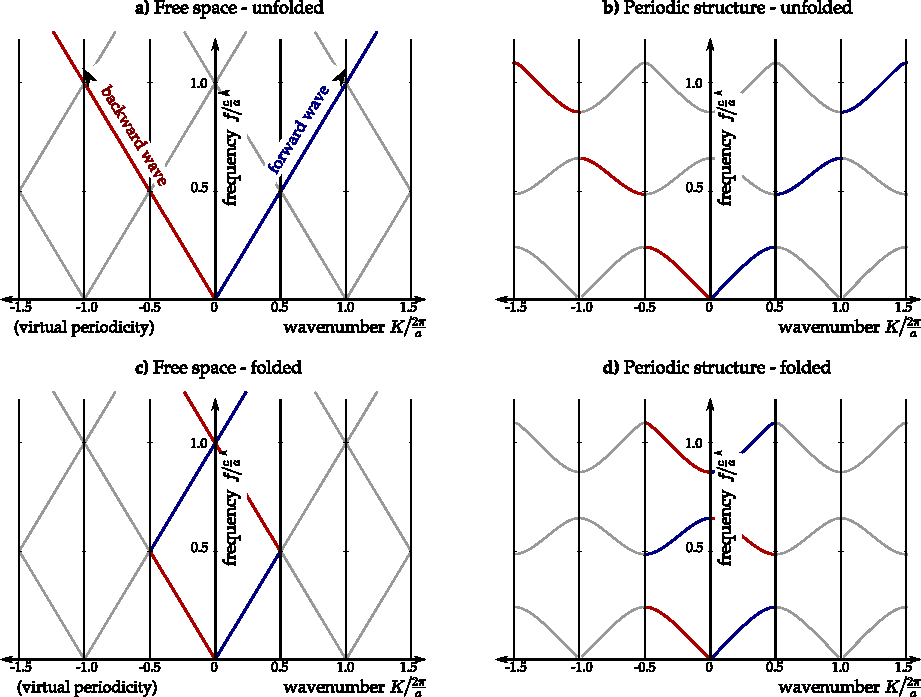
\includegraphics[width=17cm]{img/PhC_folding_illustration.pdf} 
\end{figure}
When the wavelength is less than double cell spacing, or equivalently when $2\pi c /K < 2 a$, the unit cells can scatter the forward propagating wave into the backward direction and vice versa. In an infinite periodic structure the energy transfer must be conserved, so the forward and backward waves must be of the same amplitude.\footnote{The equilibrium forward and backward wave amplitudes may, however, differ in some cases even in in infinite periodic structure. One example is when the constituent materials lose time-reversal symmetry due to static magnetic field.} We assume this also in this example with virtual periodicity. The \textit{Bloch wave} (\ref{eq_bloch}) is a product of two functions, and it gives one degree of freedom to select which part of (\ref{eq_bloch}) expresses the phase shift across one unit cell. Two different conventions are used in the literature.
\begin{enumerate}
 \item{In the \textit{unfolded} plot, the phase shift is expressed entirely by the envelope $\mathrm{e}^{\mathrm{i}Kz}$. One can always find a line coming from the front side of a unit cell to its back side, along which the mode function does not change its phase significantly $\mathbf{u(\rr)}$. In other words, the volume of the unit cell is not divided by any \textit{nodal plane} in the real part of electric field  $\mathbf{u(\rr)}$. (However, closed nodal planes within the unit cell may appear due to individual resonances.)

In vacuum, the mode function takes the simplest form, being constant $\mathbf{u(\rr)} = 1$ at all frequencies. The dispersion relation of vacuum forms a direct line as plotted in Fig. \ref{fg_phc}a.} 
 \item{The \textit{folded} plot requires $K/\left(\frac{2\pi}{a}\right) \in (-\frac{1}{2}, \frac{1}{2})$ and the remaining phase is mostly expressed by the mode function. 
Further savings of space in the plot can be made using the symmetry of the forward and backward waves, so only the positive half for $K/\left(\frac{2\pi}{a}\right) \in (0, \frac{1}{2})$ has to be plotted to describe the mode structure.} 
 \end{enumerate}
Although maybe less instructive, usually the \textit{folded} bands are plotted in the literature and they are used also in Fig. \ref{fg_1dbd}, \ref{fg_rodh} and \ref{fg_erod_radius11} below. The same approach can be used for periodic structures, where the bands are separated by band gaps, cf. Fig. \ref{fg_phc}b and \ref{fg_phc}d.
%}}}
% TODO \begin{figure} \caption{img/dispersion\_curve\_periodic\_structure.pdf}  \centering 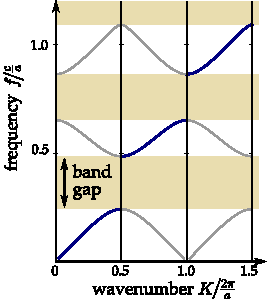
\includegraphics[width=8cm]{img/dispersion_curve_periodic_structure.pdf} \end{figure} \clearpage
% TODO \begin{figure} \caption{img/dispersion\_curve\_vacuum.pdf}  \centering 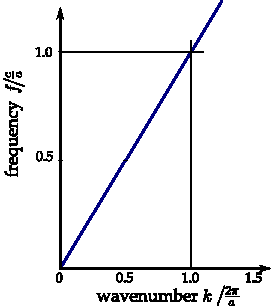
\includegraphics[width=8cm]{img/dispersion_curve_vacuum.pdf} \end{figure} \clearpage
% TODO \begin{figure} \caption{img/dispersion\_curve\_vacuum\_virtperiodic.pdf} \centering 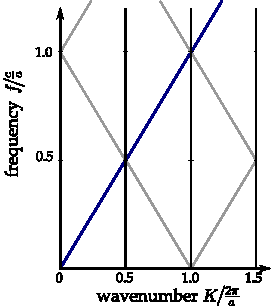
\includegraphics[width=8cm]{img/dispersion_curve_vacuum_virtperiodic.pdf} \end{figure} \clearpage


% -> K-space and isofrequency contours
% -> signal velocity, Group velocity, phase velocity and their signs \cite{Mikki}, group velocity can be negative or superluminal - no problem here?
% -> "Hopping model" -- individual oscillators with frequency more-or-less dependent on boundary conditions 
%			 (Neumann ... Gamma point ... "dE/dx=0"  vs.  Dirichlet ... M-point ... "E=0")
% -> Antiresonances -- problems with epsilon-mu approach
% -> EDB model for periodic structures

\subsection{Properties of photonic band-gaps}
% -> application of PBG, todo add references; formation: \cite{laktionov2008}
% -> zero-width case, as a transition between a mode traversing from one photonic band to another
% -> concept of nodal planes (or, more precisely, surfaces)
% -> exponential wave decay with phase difference across the cell
% -> note about how Fourier transform allows no point source to radiate energy within the bandgap
% -> PhCs with metallic/metamaterial inclusios, [Monsoriu, Lina Shi and friends]
\subsection{Physics of negative phase and/or group velocity media}
% -> homogeneous media with negative group velocity
% -> refraction on the boundary 
% -> negative group velocity and power flow [Mikki]
% -> negative index media
% -> isofrequency contours in DNG


\subsection{Homogenization}
%		"process of replacing a complex structure of subwavelength sized components with an “effective medium” with uni-
%		form properties. It is a fundamentally important notion which can be traced back to the earliest days of electro-
%		magnetic theory, to the Lorentz-Lorenz and Maxwell-Garnet effective medium models [1–3]
%			[1] J. C. M. Garnett, Phil Trans. R. Soc. A 203, 385 (1904).
%			[2] D. E. Aspnes, Thin Solid Films 89, 249 (1982).
%			[3] W. Cai and V. Shalaev, Optical Metamaterials: Fundamentals and Applications (Springer, New York, 2010).

% "Metamaterials do not bring new physical phenomena, they only force one to conscientiously review the common electrodynamics. There
% are no novel phenomena, just a novel task of homogenisation and possibly enew values of constitutive parameters"


\subsection{What are metamaterials and photonic crystals?} 
\add{
The studies of periodic electromagnetic structures is generally divided into two classes: the \textit{photonic crystals} and \textit{metamaterials}. These types of structures are formally very similar, as they are composed of 2-D or 3-D periodic array of unit cells, and the qualitative difference can be found only after the interaction with an electromagnetic wave is known. 

%The difference is in the way how the unit cell interacts with the electromagnetic field. 
In the photonic crystal (PhC), at its frequency range of operation, the effective wavelength is similar to the cell spacing and the cells scatter the propagating wave.
The energy of the resonant field is spread relatively evenly over the majority of the unit cell volume, which results in great sensitivity of the PhC behaviour to its periodicity and typically also in a high spatial dispersion. The most prominent phenomenon observed in PhC is the emergence of forbidden photonic bands around resonant frequencies, where the light can not propagate through the structure. 

On the contrary, 
the cells of a metamaterial (MM) are expected to exhibit individual resonances which should not significantly couple to each other. 
At the resonant frequencies in the metamaterials, the majority of the energy of the electromagnetic field is localised in a fraction of the unit cell volume, so that the behaviour of the metamaterial usually has only weak spatial dispersion, if any. This allows one to describe many metamaterials with acceptable precision as a homogeneous medium with a index of refraction $N(f)$, wave impedance $Z(f)$ and related effective permittivity $\varepsilon(f)=N/Z$ and permeability $\mu(f)=NZ$. 

Both types of structures exhibit the most interesting behaviour at their frequencies of resonance, but the different types of resonances define the technology and materials used to build them. The resonances in PhC rely on wave scattering, which can be easily obtained with any ordinary low-permittivity material such as silica or silicon. On the other hand, the resonances 
%but the mentioned difference has profound consequences on the behaviour of the structure. 


}
\begin{figure} \caption{img/mm-phc-diagram.pdf}  \centering 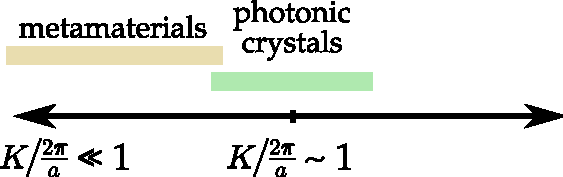
\includegraphics[width=10cm]{img/mm-phc-diagram.pdf} \end{figure} \clearpage
%% MM: HOW the light propagates.  <------>      PhC: IF the light propagates.
%% Definitions:
%% Igor Tsukerman: (Nonlocal homogenization of metamaterials by dual interpolation of fields)
%%   "metamaterials - artificial periodic structures with features smaller than the vacuum wavelength"
%% note that Veselago68 speaks about a truly *homogeneous* medium
% -> cloaking (aside from losses)
% -> superlens (aside from losses and aberration, in a hypothetical case that the MM structure can be made much finer than a detector ...)
% -> hyperlens 
% -> metasurfaces (impedance engineering, tunable properties, thin high-contrast filters)


\paragraph{Historical regards}
\paragraph{Attempt of proper definition of Metamaterials}
%% TODO
%% This is after the theory of eldn in periodic media.
%% Nonresonant metamaterials (ie. in the 1st Brillouin zone, see Juraj]
\cite{richter1995}
\cite{kadlec2008}

More detailed investigation shows that the effective-medium approach does not give accurate results when the structure is not infinite \cite{richter1995}, as is often the case. Therefore, a numerical computation using the rigorous coupled-wave analysis (RCWA) or using FDTD has to be used.

%% note Silveirinha 2007 
%% resonant metamaterials operate in the 2nd BZ (or possibly even third or higher? )
%% Think over, note the paper Dominec2014

%% PK: "The word “metamaterial” (MM) appeared first in the paper by Smith et al. in 2000 [6] where a structured material" -- is it true?

% "note that whenever a transmission is plotted, one always refers to a finite sample; in the discussion of infinite (periodic) media, 
%       only the allowed or forbidden band are to be discussed"

\section{Materials available for metamaterial construction}
\subsection{General notes}
\subsection{Dielectrics}
\subsection{Metals}
% and oxides for optical: Naik2011.pdf
\subsection{Superconductors}
\subsection{Tunable and switchable materials}
\subsection{Specifics of the terahertz range}

\mdf{
\section{TODO}

EBD theory and nonlocal electrodynamics 
\cite{krowne2007book_agran}
\cite{landau1984electrodynamics}
\cite{agranovich2006spatial}
\cite{mikki2009electromagnetic}
\cite{vinogradov2002form}
\cite{golubkov1995boundary}
\cite{agranovich2004linear}
\cite{agranovich1962crystal}

Homogenisation of nonlocal media such as wires 
\cite{capolino2009book}
\cite{silveirinha2007metamaterial}
\cite{belov2003strong}
\cite{belov2002dispersion}
\cite{lindell2001bw}
\cite{silveirinha2005homogenization}

Homogenisation issues - response to our paper from OpEx
\cite{rockstuhl2008transition}
\cite{paul2011reflection}
\cite{andryieuski2012bloch}
\cite{andryieuski2010homogenization} 
\cite{simovski2007bloch}
\cite{simovski2009material}
\cite{simovski2011electromagnetic}
\cite{mortensen2010unambiguous}

Kramers-Kronig relations in nonlocal medium
\cite{skettrup1970kramers}
\cite{kirzhnitz1976}
\cite{melrose1977generalised}
\cite{sun1989kramers}
\cite{rozanov2003}
\cite{bruleanalysis}
\cite{makarov2013kramers}
}


%Introduction
	%What is metamaterial
	%Motivation for MM
	%Motivation for THz range
%Fundamentals
%Dielectric spectra
%eps,mu -> N,Z -> reflectivity
%K-K relations
%putting two resonances near to each other annihilates their “wings”
%→ hard to make a broadband-operating passive MM
%Metal eps spectra
%different models: Drude, lossy Drude
%spatial view of E+M wave propagation  (propagating/standing wave)
%in free space
%in arbitrary electromagnetic material 
%reflection on metal surface (PEC) and on PMC
%surface plasmons, standing/propagating
%non-lossy and lossy metal (-> quasi-bound states)
%interpreting resonance (and Fano-resonance) curves
%wave in free space → s12 ampli constant, phase constantly growing; (s11 zero)
%→  in polar plot: a clockwise rotating unit vector
%reflective surface → s11 ampli constant, phase constantly growing; (s12 zero)
%simple resonance (in SRR?) 
%→  reflectivity peak
%→  losses
%in polar plot of s12: fast clockwise curl, approaching zero point, phase up-DOWN-up
%in polar plot of s11: clockwise curl starting at zero, making trip, returning to zero
%Fano resonance: requires spiral segment of curve
%case of "little fast curl 1" on "big slow curl 2"
%if fres1 = fres2 → subtractive effect, both in amplitude and phase; phase up-down-UP-down-up
%if fres1 < fres2 → …
%find out the difference between:
%two coupled broad resonances with interaction inbetween?
%Capacitive, inductive, resistive coupling?
%a “fast” and a “slow” resonance superposed?
%Two oscillators with nearly the same frequency:
%electric+electric or magnetic+magnetic → strong coupling, leads to twice curled curve in polar plot
%electric+magnetic → weak or no coupling (magnetic dipole: H field even, Efield odd; electric dipole: H field odd, E field even → may be regarded as zero inner product of the field functions)
%Scaling and non-scaling properties [Zhou PRL 2005]
%(Mode curve anticrossing)
%Babinet principle
%(Quantum states in left-handed media?)
%
%Building metamaterials: key principles
%Homogenisation
%methods, issues, desired homogenized parameters
%Metal functions
%diluted metal → Pendry1996's low frequency plasmons
%(Are cut-wire stripes useful e.g. for stable numerical simulations? They have finite eps at freq=0)
%antennae: resonator-field coupling
%metallic resonators: negative mu from SRR/Horseshoe/double-stripe
%Bianisotropy and chirality
%SRR and double-SRR
%keeping rotational-translational symmetry
%tunability
%MM impedance and coupling to free-space waves
%Mode coupling
%capacitive/resistive, behaviour, conditions, applications
%relations between MM and photonic crystal
%Higher-order Bloch modes
%
%Selected all-dielectric metamaterials
	%Mie resonances in high-permittivity microspheres
%
%Selected metalo-dielectric metamaterials
	%Aperture-array transmission
		%Wood anomaly in slit arrays
		%Wood anomaly in hole arrays
		%Standing SPP wave
	%“thin wires [8], [28], Swiss rolls [9], SRRs [9], electric SRRs (eSRRs) [29], [30], pairs of rods [10], [12], [31], pair of crosses [32], fishnets [17], [33]”
%
%== Weird ideas to elaborate ==
%* helical wire medium -> higher inductive load -> enables low plasma freq even for thicker wires
	%---> calculate FDTD
	%---> measure   TDTS with light bulb wires!
%* Possibility of standing phonon-polariton on SiC (!) 
%* try the anisotropic magnetic goo from the drawing board for children (but for electrical response)
%* find out how they could achieve negative phase speed
%* quantum point of view to negative phase/group velocity 
